See Fig. \ref{eq:myfig:solutions/1/30/}

\begin{figure}[!ht]
\centering
\resizebox{\columnwidth}{!}{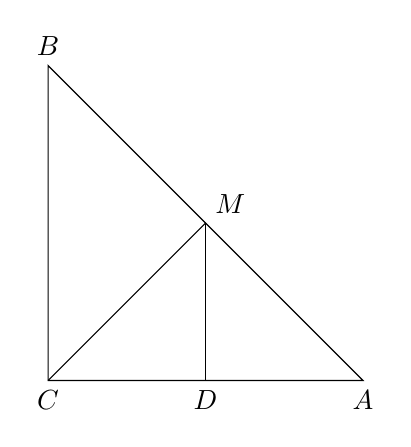
\begin{tikzpicture}
\coordinate (B) at (0,4);
\coordinate (A) at (4,0);
\coordinate (C) at (0,0);
\coordinate (D) at (2,0);
\coordinate (M) at (2,2);
\draw (A)node[below]{$A$}--(B)node[above]{$B$}--(C)node[below]{$C$}--cycle;
\draw(M)node[above right]{$M$}--(D)node[below]{$D$};
\draw(M)--(D);
\draw(M)--(C);
\tkzMarkRightAngle(B,C,A)
\tkzMarkRightAngle(A,D,M)
\tkzMarkRightAngle(C,D,M)
\end{tikzpicture}
}
\caption{Isosceles Triangle with altitudes drawn to equal sides}
\label{eq:myfig:solutions/1/30/}
\end{figure}
 Let $\vec{m}_{AC}$ and $\vec{m}_{BE}$ be direction vector of side AC and altitude BE respectively.
 \begin{align}
 \vec{m}_{AC}=\vec{A-C}\\
 \vec{m}_{BE}=\vec{B-E}
 \end{align}
Here, BE  $\perp$ AC because BE is the altitude to side AC.So,
 \begin{align}
 \vec{m}_{AC}^{T}\vec{m}_{BE}=0\\
 \vec{(A-C)}^T\vec{(B-E)}=0\\
  \vec{(A-E+E-B+B-C)}^T\vec{(B-E)}=0\\
% \begin{multlined}
\vec{(A-E)}^T\vec{(B-E)}+\norm{\vec{B-E}}^2+\\ \vec{(B-C)}^T\vec{(B-E)}=0
\\
%\end{multlined}\\
\norm{\vec{B-E}}^2+\vec{(B-C)}^T\vec{(B-E)}=0 
\label{eq:solutions/1/30/2.0.7}
\end{align}
 Let $\vec{m}_{AB}$ and $\vec{m}_{CF}$ be direction vector of side AB and altitude CF respectively.
 \begin{align}
 \vec{m}_{AB}=\vec{A-B}\\
 \vec{m}_{CF}=\vec{C-F}
 \end{align}
 Here, CF  $\perp$ AB because CF is the altitude to side AB.So,
 \begin{align}
 \vec{m}_{AB}^T\vec{m}_{CF}=0\\
 \vec{(A-B)}^T\vec{(C-F)}=0\\
\vec{(A-F+F-C+C-B)}^T\vec{(C-F)}=0\\
%\begin{multlined}
 \vec{(A-F)}^T\vec{(C-F)}+\norm{\vec{C-F}}^2+\\ \vec{(C-B)}^T\vec{(C-F)}=0
\\
%\end{multlined}\\
\norm{\vec{C-F}}^2+\vec{(C-B)}^T\vec{(C-F)}=0\label{eq:solutions/1/30/2.0.14}
 \end{align}
 Comparing equation \eqref{eq:solutions/1/30/2.0.7} and \eqref{eq:solutions/1/30/2.0.14}
\begin{multline}
\norm{\vec{C-F}}^2+\vec{(C-B)}^T\vec{(C-F)}=\\\norm{\vec{B-E}}^2+\vec{(B-C)}^T\vec{(B-E)}
\end{multline}
\begin{multline}
\norm{\vec{C-F}}^2+\vec{(C-B)}^T\vec{(C-A+A-F)}=\\
\norm{\vec{B-E}}^2+\vec{(B-C)}^T\vec{(B-A+A-E)}
\end{multline}
\begin{multline}
\norm{\vec{C-F}}^2+\vec{(C-B)}^T\vec{(C-A)}+\vec{(C-B)}^T\vec{(A-F)}=\\
\norm{\vec{B-E}}^2+\vec{(B-C)}^T\vec{(B-A)}+\vec{(B-C)}^T\vec{(A-E)}
\end{multline}
\begin{multline}
\norm{\vec{C-F}}^2+2\vec{(C-B)}^T\vec{(C-A)}=\\
\norm{\vec{B-E}}^2+2\vec{(B-C)}^T\vec{(B-A)}
\end{multline}
\begin{multline}
\norm{\vec{C-F}}^2+2(\norm{\vec{C-B}}\norm{\vec{C-A}})\cos\theta=\\
\norm{\vec{B-E}}^2+2(\norm{\vec{B-C}}\norm{\vec{B-A}})\cos\theta
\end{multline}
\begin{align}
\norm{\vec{C-F}}^2=\norm{\vec{B-E}}^2\\
\norm{\vec{C-F}}=\norm{\vec{B-E}}
\end{align}
Hence, the altitudes drawn to equal sides of isosceles triangle is equal.
